% options:
% thesis=B bachelor's thesis
% thesis=M master's thesis
% czech thesis in Czech language
% english thesis in English language
% hidelinks remove colour boxes around hyperlinks

\documentclass[thesis=M,english]{FITthesis}[2012/10/20]

\usepackage[utf8]{inputenc} % LaTeX source encoded as UTF-8

\usepackage{graphicx} %graphics files inclusion
% \usepackage{subfig} %subfigures
% \usepackage{amsmath} %advanced maths
% \usepackage{amssymb} %additional math symbols

\usepackage{listings}
\usepackage{dirtree} %directory tree visualisation
\usepackage{tablefootnote}
\usepackage{subcaption}
\usepackage{eurosym}
\usepackage{amsmath} % to center math equations
\usepackage{pifont}% http://ctan.org/pkg/pifont
\usepackage{enumitem}

\newcommand{\HRule}{\rule{\linewidth}{0.5mm}}
\newcommand{\cmark}{\ding{51}}%
\newcommand{\xmark}{\ding{55}}%

% list of acronyms
% \usepackage[acronym,nonumberlist,toc,numberedsection=autolabel,nomain]{glossaries}
%\iflanguage{czech}{\renewcommand*{\acronymname}{Seznam pou{\v z}it{\' y}ch zkratek}}{}
% \makeglossaries

\newcommand{\tg}{\mathop{\mathrm{tg}}} %cesky tangens
\newcommand{\cotg}{\mathop{\mathrm{cotg}}} %cesky cotangens

\graphicspath{ {images/} }

% % % % % % % % % % % % % % % % % % % % % % % % % % % % % % % % % % % 
% % % % % % % % % % % % % % % % % % % % % % % % % % % % % % % % % % % 
\department{Department of Computer Systems}
\title{Security Analysis of the Telegram IM}
\authorGN{Tom{\' a}{\v s}} %author's given name/names
\authorFN{Su{\v s}{\' a}nka} %author's surname
\author{Tom{\' a}{\v s} Su{\v s}{\' a}nka} %author's name without academic degrees
\authorWithDegrees{Bc. Tom{\' a}{\v s} Su{\v s}{\' a}nka} %author's name with academic degrees
\supervisor{Ing. Josef Kokeš}
\acknowledgements{TODO}
\abstractCS{TODO}
\abstractEN{TODO}
\placeForDeclarationOfAuthenticity{Prague} %where you have signed the declaration
\keywordsCS{TODO}
\keywordsEN{TODO}
\declarationOfAuthenticityOption{4} %select as appropriate, according to the desired license TODO

\begin{document}

% \newacronym{IM}{IM}{Instant Messanger}
% \newacronym{RLE}{RLE}{Run-Length Encoding}

\begin{introduction}

TODO TODO zduraznit motivaci

The human interaction and communication takes place more and more often in the digital world. This trend will most likely continue and the line between real and digital may one day disappear entirely. There is a plenty of communication solutions. Some claim themselves as very secure, some try to avoid such questions.

Today's users are picky. Instant messengers are de facto required to have both mobile and web access and more advance capabilities, such as media, voice or location sharing and the list might continue.

The surveillance disclosures emanating from the ex-NSA employee Edward Snowden showed the demand for a secure communication and number of solutions emerged. The more users share the more we realize the pitfalls of insecure communication. We shall not however forget that there is a distinction between security advertised and security actually achieved.

TODO Telegram

% This work will focus on five current Instant Messenger solutions. We will cover the messenger's history, origin, its security-related aspects and other information in order to provide the reader an insight into the security of today's modern Instant Messaging.
\end{introduction}



\chapter{Current security status of major IMs}\label{compar}

This chapter contains thorough description of five selected Instant Messengers and its security related findings. Particular software versions are mostly an estimate based on a date some findings were published and the software changelog.

\section{Selection}

We selected the following five Instant Messenger applications. The selection was based on various criterions to create a diverse mixture of messengers. The criterions among others were user base, geographical origin, authors, proclaimed security, license and price. However, we did not want to simply sort the IMs by one of those criterions. We wanted to present an indeed diverse collection. That's why we've omitted Facebook Messenger and Apple's iMessage, since the first is owned by the very same company as WhatsApp~\cite{facebookwhatsappbuy} and the later is yet another US-based company.

For ease of comparison we've decided to select messengers with support for mobile platforms. Particular software versions are mostly an estimate based on a date some findings were published and the software changelog.


\subsection{WhatsApp\protect\footnote{https://www.whatsapp.com}}

Large user base and overall popularity of the application is one of the main reasons WhatsApp is included. With 1 billion active users it is the most used messenger at the moment.\cite{whatsappusers}

\subsection{Signal\protect\footnote{https://www.whispersystems.org}}

Signal was endorsed by the community in several occasions and is by many considered as the most secure messenger. It's the only messenger completely open-sourced in this collection.

\subsection{Threema\protect\footnote{https://www.threema.ch}}

Threema is the only paid application in this selection. Furthermore Threema comes from Switzerland and may be therefore considered as an European alternative to the traditionally US-based services.

\subsection{WeChat\protect\footnote{https://www.wechat.com/en/}}

WeChat is with its 700 million active users the most used messenger in China~\cite{wechat-users}. As with Threema we include WeChat mainly for its distinct origin.

\subsection{Telegram\protect\footnote{https://www.telegram.org}}

Telegram praises itself as safer than WhatsApp. It uses its own messaging protocol MTProto and argues for its security. Telegram's clients are open-source but the server side is proprietary. The authors of Russian social network VK, Nikolaj Durov and Pavel Durov, are the creators of Telegram.


\begin{table}[htb]\centering
	\caption{Messengers}
	\label{tab:clients}
	\begin{tabular}{|l|l|l|l|l|}
		\hline
		 \textbf{Name} & \textbf{First release} & \textbf{License} & \textbf{User base} \\ \hline
		WhatsApp & January 2010 & Proprietary & 1 billion\tablefootnote{\label{foot-sep2015}As of February 2016.} \\ \hline
		 Telegram & August 2013 & GPLv2/GPLv3/Proprietary & 100 million\tablefootnote{As of February 2016} \\ \hline
		 Signal & July 2014 & GPLv3 & 10 million\tablefootnote{Signal's predecessor TextSecure as of December 2013.} \\ \hline
		 Threema & 	December 2012  & Proprietary & 3.5 million  \tablefootnote{As of June 2015.} \\ \hline
		 WeChat & January 2011 & Proprietary & 700 million\tablefootnote{As of April 2016.} \\ \hline
	\end{tabular}
\end{table}


\section{Security aspects}

The Electronic Frontier Foundation maintains a scoreboard of messaging applications' security. It evaluates messengers based on these seven criteria \cite{eff-score}:

\begin{itemize}
	\item \textbf{Are messages encrypted in transit?} All user communication is required to be encrypted. Encryption of metadata, such as phone numbers, usernames or dates, is not required.
	\item \textbf{Are messages encrypted so the provider can not access it?} All user messages need to be end-to-end encrypted, from the moment user sends a message to the moment the other party receives it. No decrypting  and re-encrypting may occur during that process. The private keys need to be generated at the endpoints, not on the centralized server. Any bulk data collection is therefore meaningless and no third-party may access the messages unless one party allows it.
	\item \textbf{Can user verify contacts' identity?} This requires a verification mechanism of the other side's identity to prevent Man-in-the-Middle attacks. 
	\item \textbf{Are past communications secure if keys stolen?} All messages need to be encrypted with routinely changed keys. The forward secrecy minimizes consequences when a private key is stolen, because the key has only a short-time validity. This criterion requires end-to-end encryption, it is therefore directly dependent on the second criterion.
	\item \textbf{Is the code open to independent review?} Sufficient amount of source-code needs to be available to perform an independent code review. This protects from unintentional encryption flaws, back doors or bugs.
	\item \textbf{Is the cryptography design properly documented?} The cryptography behind the application needs to be described in detailed documentation.
	\item \textbf{Has there been any recent code audit?} An independent security review of the application is not older than 12 months. This does not require the audit to be publicly available.
\end{itemize}

At the end of each chapter dedicated to one messenger a small note about the received score will be made.

\section{WhatsApp}\label{whatsapp}

WhatsApp is a mobile messaging application. Besides text it enables users to send pictures, videos, voice and locations. WhatsApp Messenger is available for iPhone, BlackBerry, Windows Phone, Android and Symbian\cite{whatsapphomepage}.

In February 2016 WhatsApp has reached 1 billion active users monthly and was the most used messenger to that moment \cite{whatsappusers}.

The large user base and overall popularity of the application is one of the main reasons WhatsApp is included in this comparison.

Following section describes WhatsApp's security-related incidents.

\subsection{Security-related incidents}

\subsubsection{Flaws in registration process}\label{whatsapp-registration}

WhatsApp's user identity is bound to user's phone number. In order to verify the relationship user has to enter his phone number during the first start-up. WhatsApp server then sends SMS with verification code to such number. User submits the code from the received text message and WhatsApp creates his account.  

\begin{figure}[htb]
	\centering
	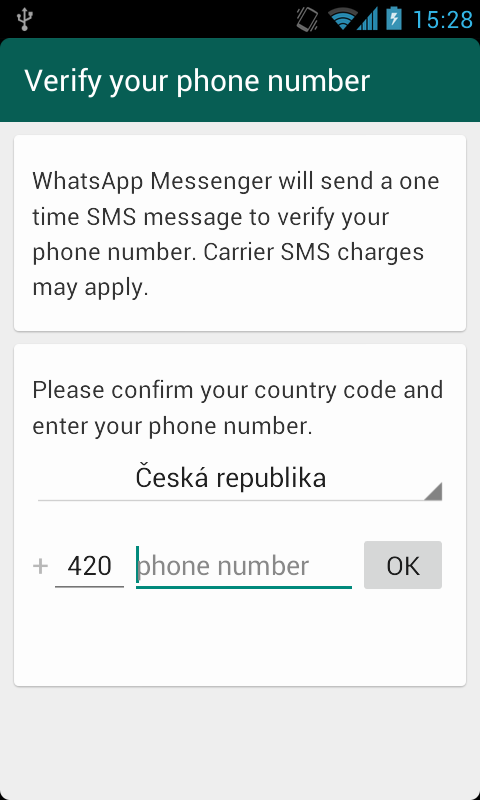
\includegraphics[width=0.4\textwidth]{whatsapp-registration.png}
	\caption{WhatsApp's registration process}
	\label{img:whatsapp_reg}
\end{figure}

Up to version 2.6.5 WhatsApp offered an alternative verification process. Instead of the user waiting for a text message, he was rather supposed to send a SMS to one of WhatsApp's phone numbers where he included his email. WhatsApp later sent verification code to the email and user verified himself with this code \cite{whatsapp-shootingthemsg}.

Serious drawbacks were found in this method in 2011 \cite{whatsapp-hijack1}. To hijack user's account attacker first opted for this method. Then using SMS spoofing service he sent SMS to WhatsApp's phone number pretending it originates from the victim. Attacker set the content of the message to an email he owned leading to WhatsApp sending the verification code to the attacker. The attacker then simply entered the code from an email and successfully hijacked the victim's account.

Following these findings another method to bypass the registration process was published. During the registration phase WhatsApp sent a request for the verification SMS to be sent to the client in HTTP request similiar to this \cite{whatsapp-shootingthemsg}:


\begin{lstlisting}[
	caption={HTTP request to dispatch SMS},
	basicstyle=\footnotesize,
	breaklines=true
]
GET [..]?to=4915143[..]&auth=659&[..] HTTP/1.1
User-Agent: WhatsApp/2.6.4 iPhone_OS/4.3.3 Device/iPhone_4
\end{lstlisting}

The request contained the final verification code in the GET parameter. That leads to a conclusion the client created the verification code, not the server, and expected user's confirmation. An attacker could simply intercept the request, retrieved the verification code and made sure the request didn't arrive to WhatsApp's servers to let the victim unaware of malicious intentions.

Attacker then created a fake HTTP OK response to let the messenger think the request was successful and entered retrieved verification code from the intercepted request. The attacker successfully hijacked the victim's WhatsApp identity and could both send and receive all his messages.

The author of the research notified WhatsApp developers beforehand and WhatsApp fixed this issue before the research was made public \cite{whatsapp-shootingthemsg}. To the date of writing this thesis WhatsApp doesn't offer discussed verification method anymore.


\subsubsection{Password generation}

WhatsApp uses lightly modified version of XMPP \cite{whatsapp-xmpp}. During the registration process it creates a username based on the user's phone number. In newer versions than 2.10 the password is generated on server's side \cite{whatsapp-imei}. However, older versions used the phone's IMEI  number as password \cite{whatsapp-imei, whatsapp-imei2}.

\begin{lstlisting}[caption={Pseudo-code of password generation on Android}]
md5(revert('IMEI')) 
\end{lstlisting}

Any phone number -- IMEI pair was therefore all an attacker needed to send messages on victim's behalf. Numerous applications are collecting plenty of user data and the IMEI and phone number might be among them. Any database leak with such information would lead directly to large accounts abuse.

\subsubsection{Messages encryption}

Up to version approximately 2.8 WhatsApp did not use any message encryption. The messenger used port 443 (commonly used for HTTPS) to send content, however it did not encrypt anything \cite{whatsapp-plaintext}. Using a simple network sniffer like Wireshark attacker was able to read all user's messages.

On May 2012 an application called ``WhatsAppSniffer'' had been released  \cite{whatsapp-sniffer}\cite{whatsapp-sniffer2}. It abused described flaw and enabled attacker to see victim's messages in easy and lucid user interface.


\begin{figure}[htb]
	\centering
	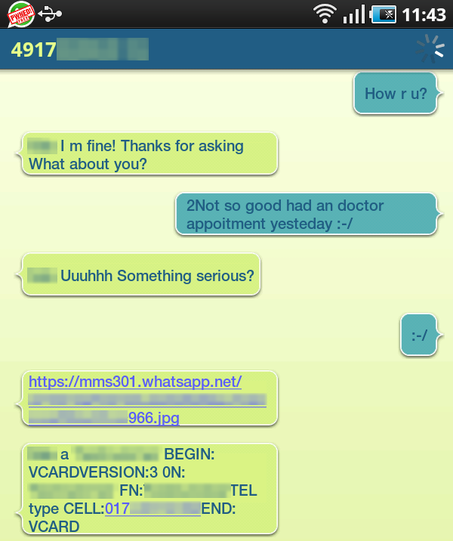
\includegraphics[width=0.4\textwidth]{whatsapp-sniffer.png}
	\caption{WhatsAppSniffer \cite{whatsapp-sniffer2}}
	\label{img:whatsapp_sniffer}
\end{figure}


On August 2012 WhatsApp started to use some sort of encryption. The developers did not reveal which protocol they use or any other information. Reports showed that simple message sniffing, as described in previous chapter, seized to work \cite{whatsapp-sniffernomore}. Some sources claim the  RC4 stream cipher was used for encryption \cite{whatsapp-rc4}\cite{whatsapp-rc42}.

On November 18, 2014, Open Whisper Systems, the creators behind Signal messenger, announced a partnership with WhatsApp. The partnership should have escalated into incorporating OWS' encryption protocol to WhatsApp bringing end-to-end encryption to all WhatsApp clients. Open Whisper Systems stated: \emph{``we are moving quickly towards a world where all WhatsApp users will get end-to-end encryption by default.''}. \cite{openwhisperwhatsapp}

WhatsApp confirmed this partnership, however did not comment it any further nor offered any further information. No additional information from Open Whisper Systems' side had been released as well. WhatsApp's FAQ currently only briefly states \emph{``WhatsApp communication between your phone and our server is encrypted.''}\cite{whatsapp-faq}.

On April 2015, \emph{heise.de} investigated the current state of WhatsApp's encryption. The journalists were sniffing messages using the Man-in-the-Middle technique. They showed that Android versions used end-to-end encryption and that the messages ``\emph{were encrypted according to the TextSecure protocol}''\cite{whatsapp-encstate}. However, during testing the iOS client they concluded the messages weren't protected in such manner. Finally, they concluded they are unsure whether end-to-end encryption was actually used in all cases.

TODO WhatsApp released white paper

\subsection{EFF's secure messaging score}

At the time of writing, WhatsApp has two points out of seven in the EFF's secure messaging scorecard \cite{eff-score}.

\begin{table}[htb]
	\centering
	\caption{WhatsApp's secure messaging score}
	\label{my-label}
	\begin{tabular}{|l|l|}
		\hline
		Are messages encrypted in transit? & \cmark \\\hline
		Are messages encrypted so the provider can not access it? & \xmark \\ \hline
		Can user verify contacts' identities? & \xmark \\ \hline
		Are past communications secure if keys stolen? & \xmark \\ \hline
		Is the code open to independent review? & \xmark \\ \hline
		Is the cryptography design properly documented? & \xmark \\ \hline
		Has there been any recent code audit? & \cmark \\ \hline
	\end{tabular}
\end{table}


\section{Signal}

Signal is an open-source voice calling and messaging application. It is available for Android and iOS. Its messages are end-to-end encrypted. During a voice calls simple identity check is available when a given word is included by both sides in the call.

Signal uses its own Signal Protocol (previously called \emph{Axolotl}) based on cryptographic primitives such as Elliptic Curves (Curve25519), AES and HMAC-SHA256. \cite{signal-bochum} As mentioned in Section~\ref{whatsapp} WhatsApp might use the very same protocol. TODO - od začátku 2016 ho opravdu ofiko používá

\subsection{Security-related incidents}

In late 2014 \emph{Der Spiegel} published articles claiming NSA considered Signal's encrypted voice calling used with other tools as a catastrophic to theirs surveilance missions.\cite{signal-spiegel} Edward Snowden recommended Signal on various occasions.\cite{signal-snowden}\cite{signal-snowden2}

A research team from Ruhr University Bochum provided a security analysis \emph{``How Secure is TextSecure?''} of the former Signal version.\cite{signal-bochum} They came to a conclusion that the protocol is susceptible for an Unknown key-share attack and proposed a mitigation. If such patch applied they concluded Signal as secure.

Up to this date no other security-related incidents or analysis of Signal messenger are known.

\subsection{EFF's secure messaging score}

Signal fulfilled all the requirments in the EFF's secure messaging scorecard and received a full score. \cite{eff-score}

\begin{table}[htb]
	\centering
	\caption{Signal's secure messaging score}
	\label{my-label}
	\begin{tabular}{|l|l|}
		\hline
		Are messages encrypted in transit? & \cmark \\\hline
		Are messages encrypted so the provider can not access it? & \cmark \\ \hline
		Can user verify contacts' identities? & \cmark \\ \hline
		Are past communications secure if keys stolen? & \cmark \\ \hline
		Is the code open to independent review? & \cmark \\ \hline
		Is the cryptography design properly documented? & \cmark \\ \hline
		Has there been any recent code audit? & \cmark \\ \hline
	\end{tabular}
\end{table}


\section{Threema}

Threema is a paid IM application available for all three major platforms -- Android, iOS and Windows Phone. Text messaging, multimedia, locations, voice messages and file sharing are supported. Threema is developed in Switzerland and all servers are located in the very same place.

Threema is a paid application. As of June 2016 the price was set to \euro2.5. Threema is using user IDs and linking user's phone number and email address is not required.

\subsection{Security-related incidents}

In August 2015, Threema was auditted by an external company. The Threema documentation states \cite{threema-audit}: \emph{``The result confirms that Threema's concepts fully meet the requirements for secure and trustworthy instant messaging.''} The full audit is available on Threema's web page.

The main point of Threema's criticism is considered with its closed-source nature therefore the inability to verify its source code.

There are no other security analysis.

\subsection{EFF's secure messaging score}

In the EFF's comparison Threema missed a single point for not completing an indenpendent code review. \cite{eff-score}

\begin{table}[htb]
	\centering
	\caption{Threema's secure messaging score}
	\label{my-label}
	\begin{tabular}{|l|l|}
		\hline
		Are messages encrypted in transit? & \cmark \\\hline
		Are messages encrypted so the provider can not access it? & \cmark \\ \hline
		Can user verify contacts' identities? & \cmark \\ \hline
		Are past communications secure if keys stolen? & \cmark \\ \hline
		Is the code open to independent review? & \xmark \\ \hline
		Is the cryptography design properly documented? & \cmark \\ \hline
		Has there been any recent code audit? & \cmark \\ \hline
	\end{tabular}
\end{table}


\section{WeChat}

WeChat is a mobile messenger developed in China. It's available to all major mobile platforms including iOS, Android, Windows Phone and BlackBerry. Besides regular text messages WeChat offers media, location, video sharing and even games. As of May 2016, WeChat had 700 million active users \cite{wechat-users}.

A special business versions of WeChat was introduced in April 2016 named Enterprise WeChat focused on companies communication offering few additional features.

\subsection{Censorship}

The Internet censorship of China blocks extensive amount of web sites including web giants such as Facebook, Twitter or Google \cite{china-twitter}\cite{china-facebook}.

Since WeChat's servers are located in China it is subjected to such restrictions. Users are required to agree and obey specific rules such as \emph{``upholding the socialist system, social morality and authenticity of information''} \cite{china-imblocking}. The reasons for such actions are supposed to build a clean cyberspace and to ensure the national security \cite{china-blocking2}.

\subsection{Security-related incidents}

WeChat operators are capable of accessing messages, contacts and even user's location. Numerous states including United States, India and China itself expressed concerns over WeChat being a threat to their national security issues \cite{wechat-states}.

\subsubsection{XcodeGhost malware}

In 2015 Apple reported WeChat was infected with XcodeGhost malware \cite{wechat-xcodemalware}. The malware was able to obtain user device information, read clipboard, prompting alert dialog and others. Apple claimed the malware was not able to perform any real damage and could not access any user data. 

\subsection{EFF's secure messaging score}

Regrettably WeChat was not included in the EFF secure messaging survey.


\section{Telegram}

Telegram is instant messaging service enabling users to send messages, photos, videos, stickers and files. Telegram describes itself as fast and secure solution for instant messaging and claims to be safer than WhatsApp. Compared to WhatsApp, Telegram is more cloud-based, it stores all messages on its servers and sync them with all user's devices.\cite{telegramfaq}

Nikolaj and Pavel Durov are the authors of Telegram. After leaving the  social network VK Pavel Durov founded, they focused on creating safe forms of communication leading to Telegram.

Telegram provides two modes of messaging. Besides the regular chat Telegram provides ``secret chats''. Secret chat messages are encrypted using end-to-end encryption and are not stored on Telegram's servers\cite{telegramfaq}.

\begin{figure}[htb]
	\centering
	\label{A}
	\begin{subfigure}[b]{0.4\textwidth}
		\centering
		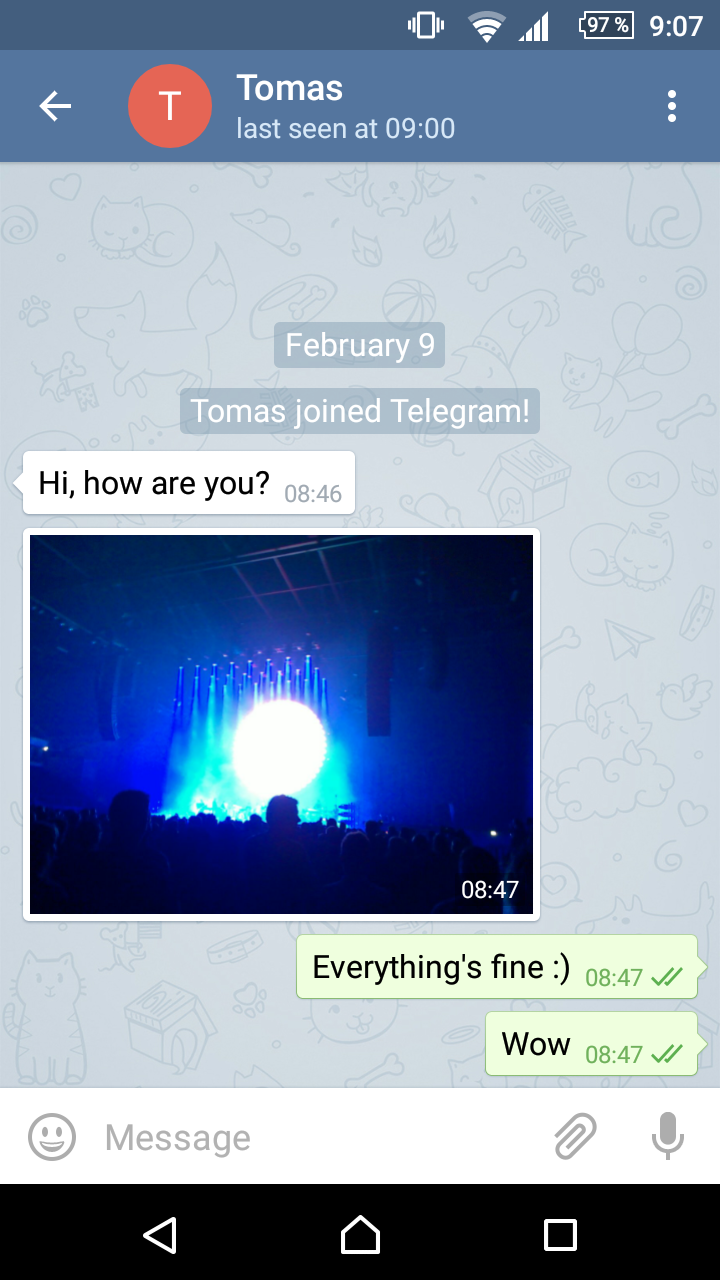
\includegraphics[width=0.9\textwidth]{telegram-regular.png}
		\caption{Regular chat}
		\label{img:telegram:regular}
	\end{subfigure}
	\hfill
	\begin{subfigure}[b]{0.4\textwidth}
		\centering
		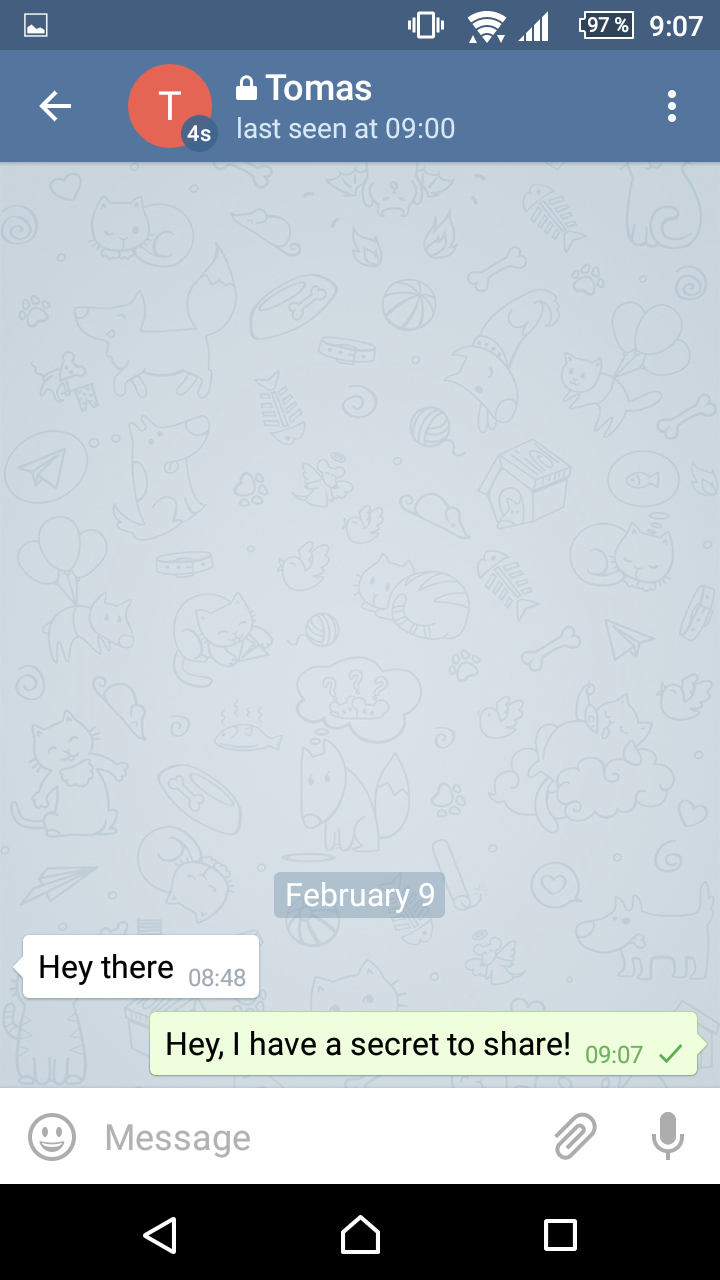
\includegraphics[width=0.9\textwidth]{telegram-secret.png}
		\caption{Secret chat}
		\label{img:telegram:secret}
	\end{subfigure}
	\caption{Telegram chat modes}
\end{figure}

Similar to WhatsApp user can contact someone using his phone number but Telegram provides classical username approach as well. User needs to know the recipient's phone number or Telegram username in order to communicate with him.

All clients are licensed under GPLv2 or GPLv3 license, the server-side part of Telegram is closed-sourced and proprietery \cite{telegram-server}.

In 2015 Brazilian judiciary ordered WhatsApp to shut down for 48 hours. During this event, which was finally lowered to only 12 hours, Telegram welcomed 5 million new users.\cite{whatsappbrazil} It may be therefore considered as a direct competitor to WhatsApp.

In May 2015 Telegram had 62 million active users \cite{telegram-users}.


\subsection{Security-related incidents}

\subsubsection{SMS authentication}

In Section~\ref{whatsapp-registration} we described how the WhatsApp's registration process using SMS works. Telegram works on a similar basis and allows as well logging in using just a simple SMS.

Those are fully readable for mobile network operators which may and usually do cooperate with the corresponding government. Furthermore SMS can be intercepted using inexpensive IMSI catchers. If an attacker is able to steal the authenticating SMS he is able to login on his behalf. Worse, Telegram stores the whole user's message history, hence it allows the attacker to read old messages as well.

Early 2016 was shown this was a legitimate concern \cite{telegram-smsiran}. Some Telegram users experienced their accounts being erased and blamed Telegram to enforce political censorship. Telegram denied. Russian activist Oleg Kozlovsky described in its Facebook post \cite{telegram-russia} how his account was allegedly hacked.

First the Russia's mobile operator disabled SMS service on Oleg's phone number. Upon the disconnection, the attacker tried to log into victim's Telegram account. Since intercepting the SMS is all the attacker needs he simply entered the authorization code he sniffed and got full access to Oleg's account. Telegram recommended to turn on two-factor authentication for additional security.

These concerns raise serious questions if SMS authentication is a security-wise valid instrument.

\subsubsection{Cracking Contest}

On November 4, 2014, Telegram published contest with a winning price \$300,000 for cracking its encryption. The contest became quite known in the community and probably provided a bit of advertisement for Telegram.

The contest remained unsolved until his closure. Number of authors considered it rigged and stated that the contest does not provide any prove of Telegram's overall security whatsoever.\cite{telegramcontestfail}\cite{telegramcontestfail2}

\subsection{EFF's secure messaging score}

As mentioned Telegram has two types of messages. Telegram is therefore evaluated twice by the EFF.

\subsubsection{Telegram regular chats}

\begin{table}[htb]
	\centering
	\caption{Telegram regular chat's secure messaging score}
	\label{tab:telegram-regular-eff}
	\begin{tabular}{|l|l|}
		\hline
		Are messages encrypted in transit? & \cmark \\\hline
		Are messages encrypted so the provider can not access it? & \xmark \\ \hline
		Can user verify contacts' identities? & \xmark \\ \hline
		Are past communications secure if keys stolen? & \xmark \\ \hline
		Is the code open to independent review? & \xmark \\ \hline
		Is the cryptography design properly documented? & \cmark \\ \hline
		Has there been any recent code audit? & \cmark \\ \hline
	\end{tabular}
\end{table}


\subsubsection{Telegram secret chats}

\begin{table}[htb]
	\centering
	\caption{Telegram secret chat's secure messaging score}
	\label{tab:telegram-secret-eff}
	\begin{tabular}{|l|l|}
		\hline
		Are messages encrypted in transit? & \cmark \\\hline
		Are messages encrypted so the provider can not access it? & \cmark \\ \hline
		Can user verify contacts' identities? & \cmark \\ \hline
		Are past communications secure if keys stolen? & \cmark \\ \hline
		Is the code open to independent review? & \cmark \\ \hline
		Is the cryptography design properly documented? & \cmark \\ \hline
		Has there been any recent code audit? & \cmark \\ \hline
	\end{tabular}
\end{table}







\chapter{Cryptography behind Telegram}\label{telegramcrypto}

Telegram authors decided to craft a brand new encryption scheme supposedly to achieve better delivery times and stability, MTProto. For simplicity we will focuse on Telegram's secret chats messaging only. The analysis is mainly based on \cite{telegram-aarhus} and on the official Telegram documentation. 


\subsection{Initialization}\label{crypto-initialization}

Upon the first lunch of Telegram application user needs to enter and verify its telephone number. Then the client establishes a secure connection with one of the Telegram's servers. This connection is based on RSA, simple proof-of-work calculation, Diffie-Hellman key exchange and finally AES-IGE encryption. This key is subsequently used for any client-server communication and regular chats. As mentioned, we want to focus primarily on secret chats, hence this key exchange is not described into more details.


\subsection{Key exchange}\label{crypto-keyexchange}

Now we'll describe the key exchange during the secret end-to-end encrypted messaging.

The exchange performs traditional Diffie-Hellman key exchange (DH). The DH parameters are received from the servers using the connection described previously in \ref{crypto-initialization}. The client receives $p$ and $g$ and should check the following conditions are met:

\begin{itemize}
	\item $p$ is a safe prime, meaning $q = \frac{p-1}{2}$ needs to be prime as well
	\item $2^{2047} < p < 2^{2048}$
	\item $g$ generates a cyclic subgroup of prime order $q$
\end{itemize}

We compared these requirements with the FIPS 186-4 publication concerning Digital Signature Algorithm and concluded the Telegram requires similar conditions with only minor distinctions.

Now suppose user $A$ initiates secret chat with $B$:

\begin{enumerate}
	\item $A$ computes a random 2048-bit number $a$ and sets $g_a = g^a \bmod p$\label{enum:DH-a}
	\item $B$ receives the request on all of its authorized devices and an exclusive one accepts it
	\item $B$ generates random $b$ and sets $g_b = g^b \bmod p$\label{enum:DH-b}
	\item Both users calculate the master key $K = g_a^b \bmod p = g_b^a \bmod p$. We denote this master key \texttt{auth\_key}
\end{enumerate}

If the length of \texttt{auth\_key} is lower than 2048 bits, leading zeros are added as padding.

In the steps \ref{enum:DH-a} and \ref{enum:DH-b} both clients are to check $1 < g_a, g_b < p-1$ and is recommended to verify $2^{2048-64} < g_a, g_b < p - 2^{2048-64}$ as well. Worth mentioning, the client generates its \emph{a} (\emph{b} respectively) in the following way:
\begin{gather*}
a = r_{client} \oplus r_{server}
\end{gather*}

Where $r_{client}$ is a 2048-bit random integer generated on the client side and $r_{server}$ is 2048-bit random integer generated on the server side. These values are then XORed constructing the client's secret value. This is performed to mitigate the client's poor capabilities to generate a cryptographically secure random number as concerned Android in August 2013 \cite{telegram-android-securerandom}.

\begin{figure}[htb]
	\centering
	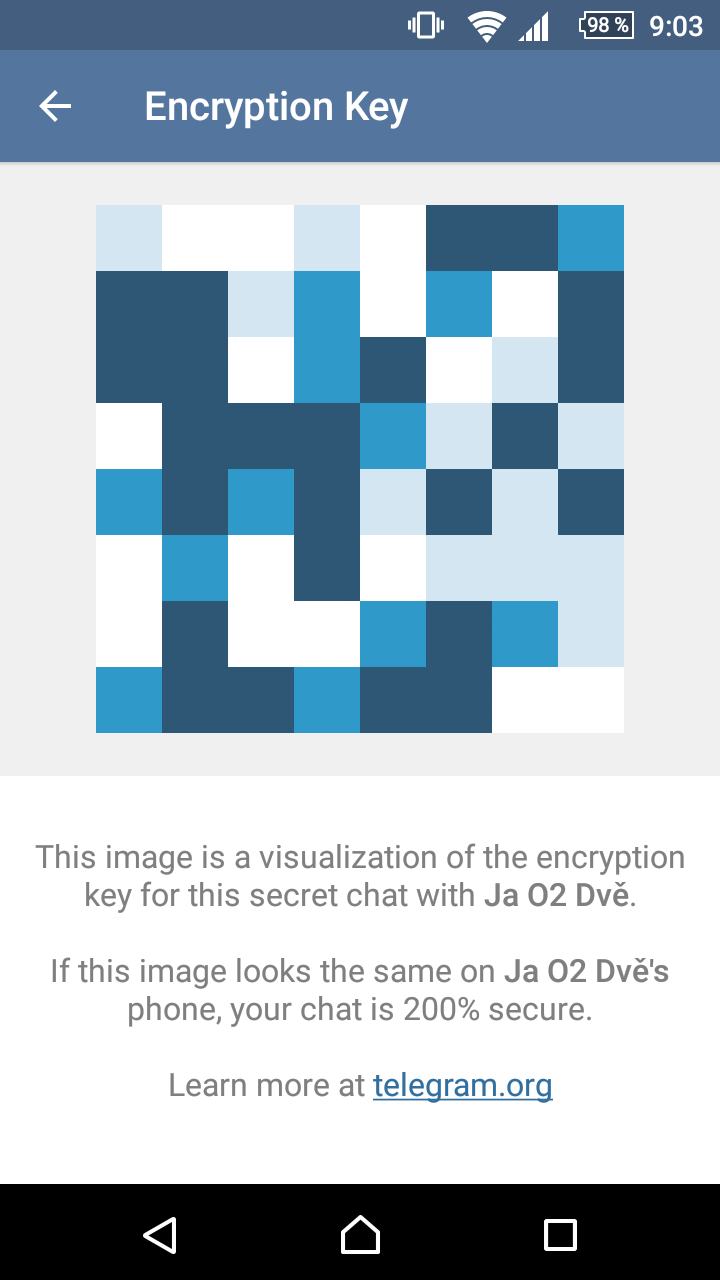
\includegraphics[width=0.4\textwidth]{telegram-keybox.png}
	\caption{Encryption key visualization}
	\label{img:telegram-keybox}
\end{figure}

The DH by itself does not provide any authentication of the communicating parties and is therefore susceptible to an active Man-in-the-Middle attack. To mitigate this issue the user is provided with an option to display counterpart's encryption key. Telegram creates a white-blue box to visualize the key as may be seen on Figure~\ref{img:telegram-keybox}. To make sure no malicious mediator is present users are supposed to meet in person and verify the keys are identical.

The visualisation used to be based on a 128-bit fingerprint\footnote{Not to be confused with the 64-bit \texttt{auth\_key\_id} fingerprint.} of the secret key. An~article presented in January 2015 showed \cite{telegram-264} that when the attacker forces (e.g. socially engineers) both sides to initiate the secret chat, a MiM attack is possible only with $2^{64}$ operations, rather than $2^{128}$, based on the Birthday paradox. The article claims the attack is possible for a well financed adversary and estimates the attack to cost tens of millions USD. Telegram's FAQ addresses this issue and states its cost is around a trillion dollars to achieve a result in one month. Nevertheless, Telegram later decided to use additional 160 bits from the key summing up to 288 bits \cite{telegram-techfaq}. This improvement should make this attack impossible.

The article as well reasons that in real-world scenario the users don't actually meet to verify the key. Most of them probably ignore the verification whatsoever, some send the image via regular chat or using another -- possibly insecure -- channel.

To accomplish the Perfect Forward Secrecy model the key is renegotiated each time it has been used for more than 100 messages or has been used for more than one week. For the renegotiation the already established chat is used in order to send the $g_a$ and $g_b$ values. The server does not help with the randomness here and the same DH parameters are used. The \emph{auth\_key} visualization does not change and is therefore based on the first negotiated key.

Finally, a fingerprint of the exchanged \texttt{auth\_key} is created labeled as \texttt{auth\_key\_id}. It is crafted from the last 64 bits of SHA-1(\texttt{auth\_key}).

TODO Trust on first use?


\subsection{Payload}

With the key negotiated we may now focus on the message encryption itself. First, let's describe the content of a single message, further referred to as a payload.

The cornerstone of the payload is the \textbf{decryptedMessage} object depicted on Figure \ref{img:decrypted-message} which contains:

\begin{figure}[htb]
	\centering
	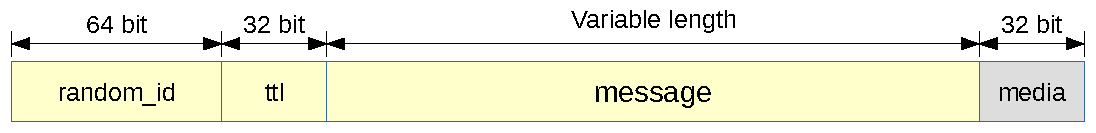
\includegraphics[width=1\textwidth]{decrypted-message.pdf}
	\caption{The \texttt{decryptedMessage} object containing the message itself and accompanied by other settings.}
	\label{img:decrypted-message}
\end{figure}

\begin{itemize}
	\item \texttt{random\_id} random value assigned by the author to identify the message; also sent as a plaintext
	\item \texttt{ttl} message lifetime\footnote{User may set a message lifetime. After such time passes Telegram deletes it.}
	\item \texttt{message} the actual text of a message
	\item \texttt{media} header used for media transfers
\end{itemize}

Throughout this paper we assume that no media attachments are present and therefore the \texttt{media} attribute is always empty. The \texttt{decryptedMessage} object is further wrapped in \texttt{decryptedMessageLayer} which adds the following fields:

\begin{figure}[htb]
	\centering
	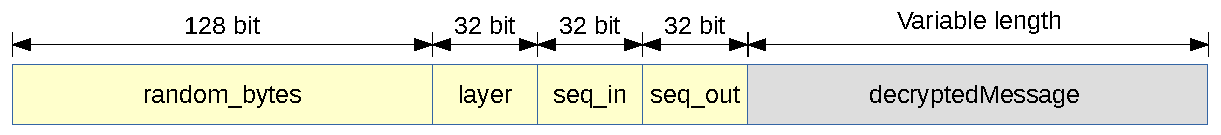
\includegraphics[width=1\textwidth]{decrypted-message-layer.pdf}
	\caption{The \texttt{decryptedMessageLayer} object contains random bytes, protocol version, sequence numbers and the \texttt{decryptedMessage} object.}
	\label{img:decrypted-message-layer}
\end{figure}

\begin{itemize}
	\item \texttt{random\_bytes} 120 random bits generated by the author followed by 8 bits to specify the length of it in bytes.
	\item \texttt{layer} version of the protocol
	\item \texttt{seq\_in} counter for incoming messages
	\item \texttt{seq\_out} counter for outgoing messages
\end{itemize}

TODO zkontrolovat, pripsat nekonzistence s danskou diplomkou? Pokud opravdu jsou

This payload is then serialized as an array of bytes and prepared to be encrypted.

\subsection{Encryption}\label{telegram-enc}

First, the message key \texttt{msg\_key} is calculated. It is composed of the first 128 least significant bits of the SHA-1 hash of the payload to be encrypted. Next, the array is padded with 0-96 random bits in order to be divisible by the AES block size -- 128 bits.

This \texttt{msg\_key} along with the \texttt{auth\_key} described in Section \ref{crypto-keyexchange} are taken as input into the Key Derivation Function (KDF) which performs number of SHA-1 hashes and truncation yielding two 256-bit values: the AES key and the IGE initialization value (IV) used for encrypting this particular message.

\begin{figure}[htb]
	\centering
	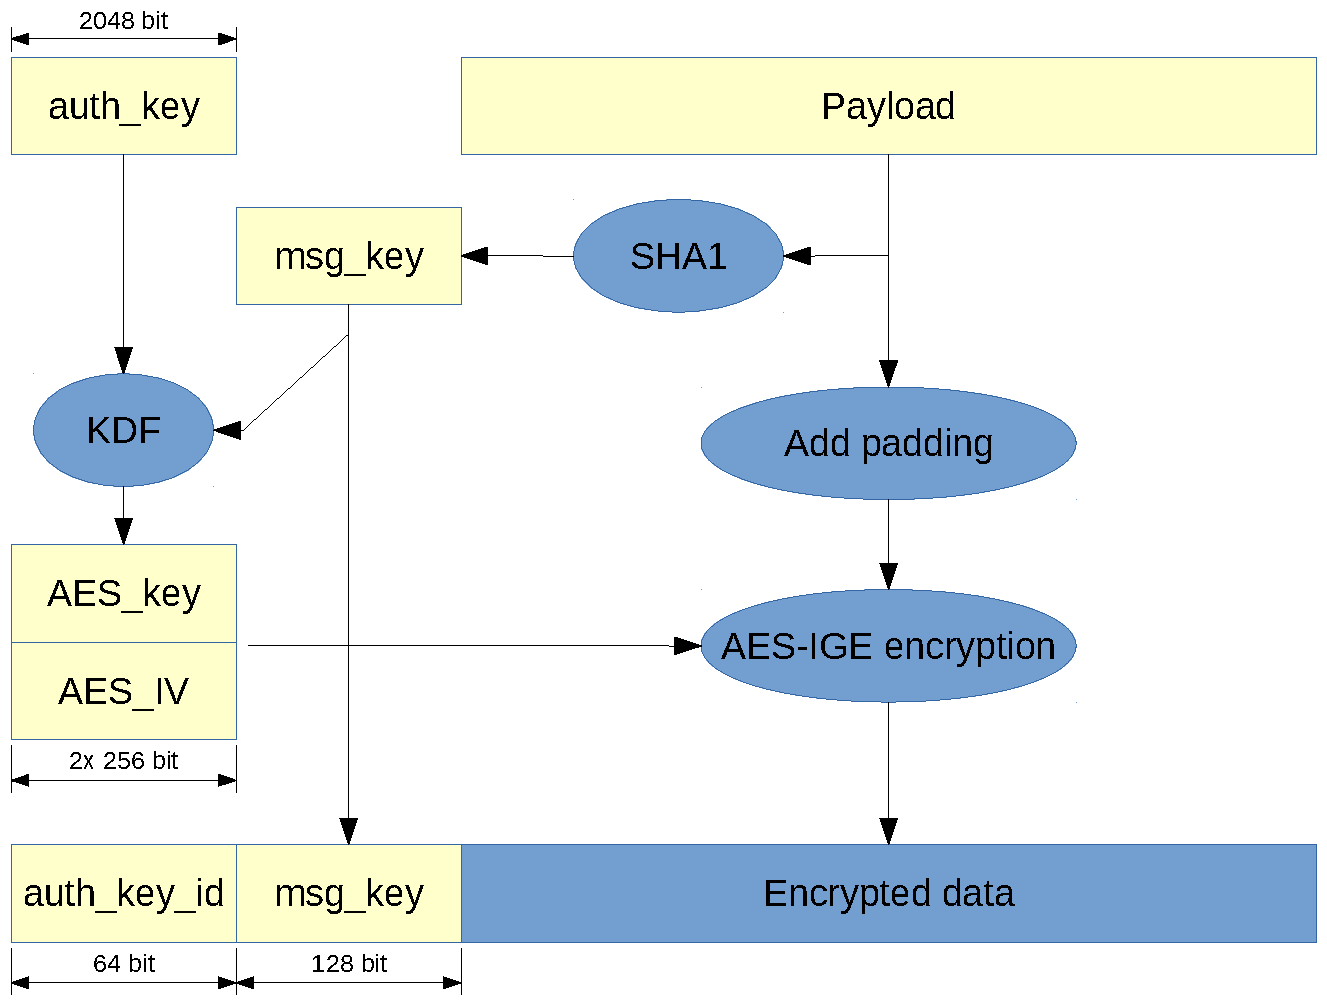
\includegraphics[width=1\textwidth]{mtproto-encflow.pdf}
	\caption{MTProto encryption flow \cite{telegram-aarhus}}
	\label{img:telegram-encflow}
\end{figure}

Two other values are added at the top of the encrypted data array: the already mentioned \texttt{msg\_key} and the \texttt{auth\_key\_id} described in Section \ref{crypto-keyexchange}. The client sends the message via the \textbf{messages.sendEncrypted} method providing these three parameters:

\begin{itemize}
	\item \texttt{peer} secret chat ID to identify the users
	\item \texttt{random\_id} unique client message ID sent encrypted in the \textbf{decryptedMessage} object as well
	\item \texttt{data} the encrypted data, \texttt{msg\_key} and \texttt{auth\_key\_id} combined in one byte array
\end{itemize}

\subsubsection{Advanced Encryption Standard}

The Advanced Encryption Standard (AES) is a symmetric block cipher with key lengths of 128, 192 and 256 bits respectively and block size of 128 bits. Telegram uses 256 bit key. AES is currently the most widely used symmetric cipher and is used in many internet standards such as IPsec, TLS, SSH and many others.

AES was selected through a worldwide open competition and finally defined in the FIPS-197 publication by the US National Institute of Standards and Technology (NIST) in 2001. As of today, AES is secure against brute-force attacks and no reasonable analytic attacks are currently known \cite{understanding-crypto}.

\subsubsection{Infinite Garble Extension}

Infinite Garble Extension (IGE) is a lesser-known block cipher mode. It is shown on Figure \ref{img:telegram-ige-enc} and defined by the following formula \cite{telegram-openssl-ige}:

\begin{gather*}
c_i = f_K(m_i \oplus c_{i-1}) \oplus m_{i-1}
\end{gather*}

where $f_K$ stands for the encrypting function with key $K$ (AES in our case) and $i$ goes from 1 to $n$ -- the number of plaintext blocks.

Careful reader notices that for the first output block we need two initialisation values $m_0$ and $c_0$. Both values are taken from the IV described earlier. The original paper described $m_0$ as a random block and $c_0$ its encrypted counterpart. The OpenSSL implementation however, uses a more general implementation where both $m_0$ and $c_0$ are provided by the user \cite{telegram-openssl-ige}.

\begin{figure}[htb]
	\centering
	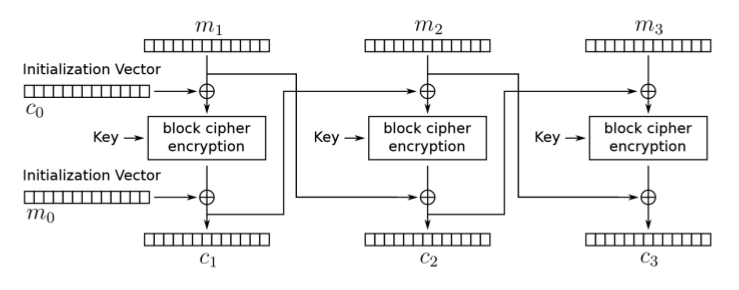
\includegraphics[width=1\textwidth]{telegram-ige-enc.png}
	\caption{IGE mode of operation \cite{telegram-aarhus}}
	\label{img:telegram-ige-enc}
\end{figure}


\subsection{Decryption}

Before the decryption process starts the \texttt{auth\_key\_id} is validated. The receiver's \texttt{auth\_key\_id} needs to match the value the sender appended to the byte array. If the values differ the whole message is discarded.

\begin{figure}[htb]
	\centering
	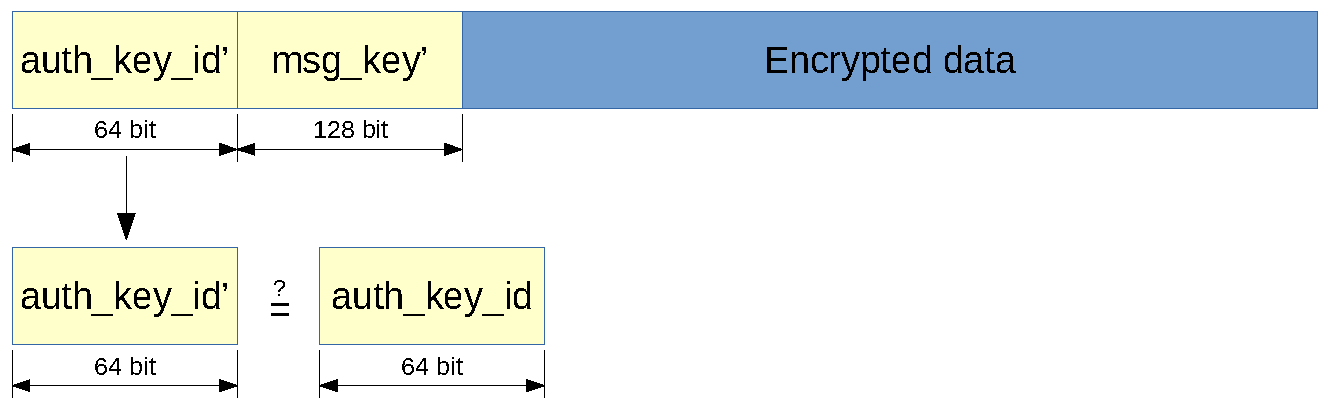
\includegraphics[width=0.9\textwidth]{mtproto-auth-key.pdf}
	\caption{Before the decryption process starts the \texttt{auth\_key\_id} values are checked.}
	\label{img:telegram-decflow}
\end{figure}

The decryption process is plainly the encryption process in reverse. The KDF yields the AES key and IV values used for decrypting the data. The padding is stripped and the SHA-1 of the payload generates \texttt{msg\_key} which is compared to \texttt{msg\_key'}. The whole process is lucidly visualized on Figure \ref{img:telegram-decflow}.

\begin{figure}[htb]
	\centering
	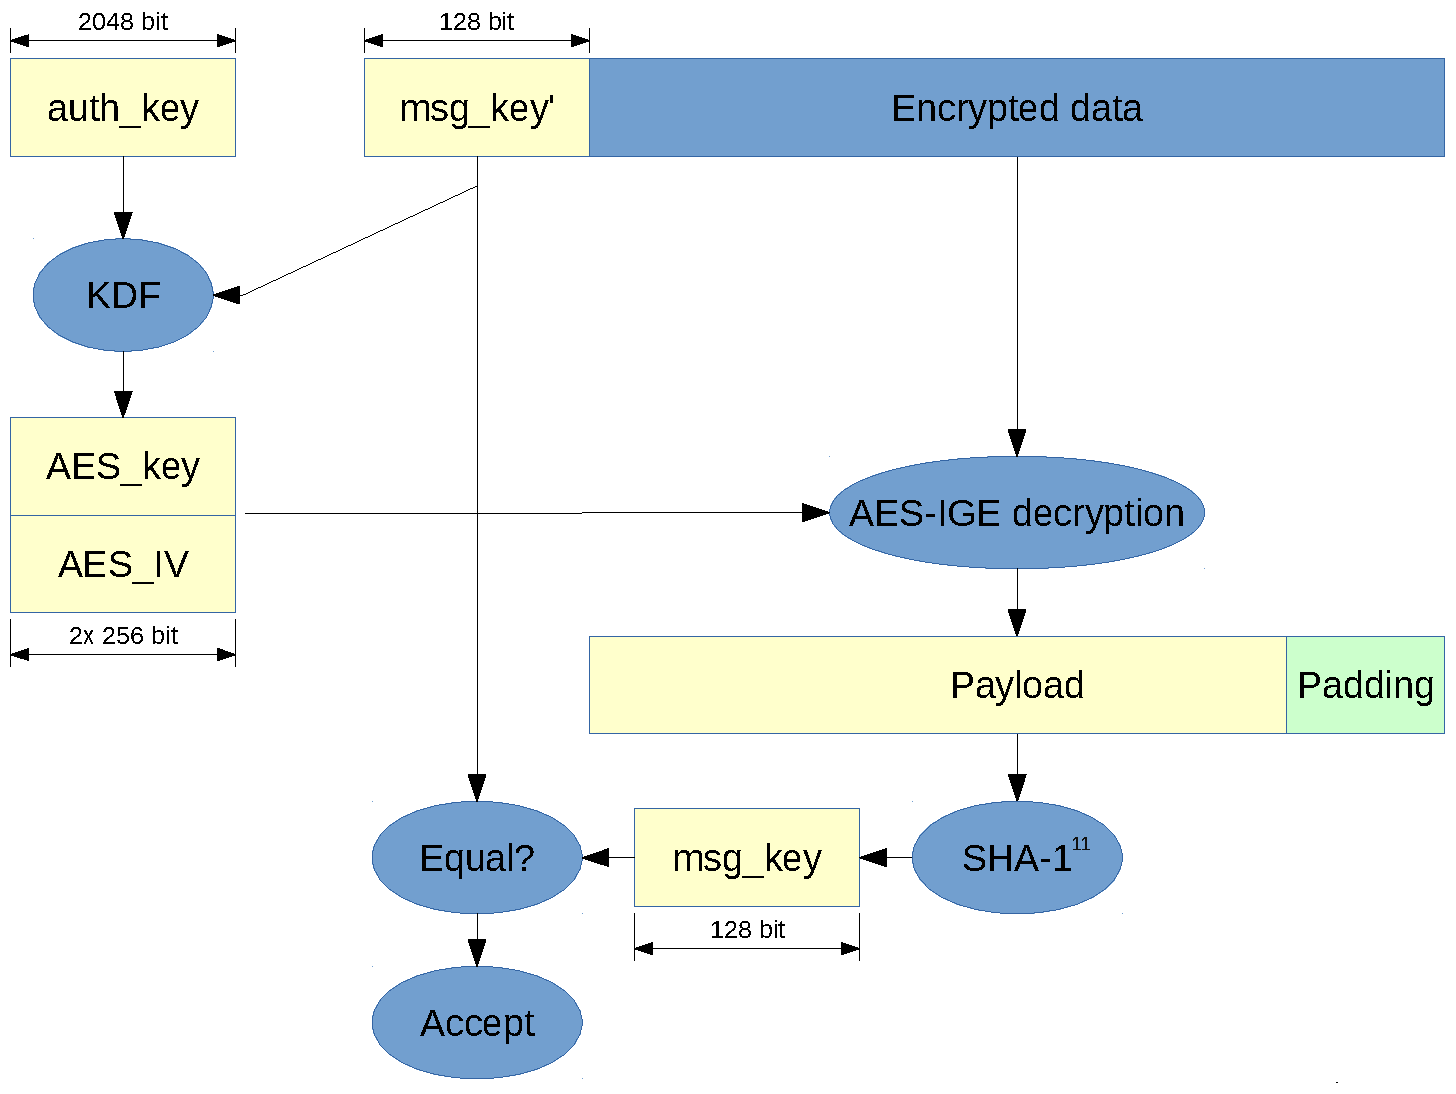
\includegraphics[width=1\textwidth]{mtproto-decflow.pdf}
	\caption{The KDF produces the AES key and IV from the \texttt{auth\_key} and received \texttt{msg\_key'}. The SHA-1 of the decrypted payload generates \texttt{msg\_key} which is compared to \texttt{msg\_key'} and only then accepted.}
	\label{img:telegram-decflow}
\end{figure}

\chapter{TODO}

\subsection{SHA-1}

Telegram architects chosed to use SHA-1 because of its low resource consumption. SHA-1 is however, cryptographically broken in some scenarios \cite{telegram-sha1}. The Bruce Schneier's blog claims \cite{telegram-sha1}: \emph{``A collision attack is therefore well within the range of what an organized crime syndicate can practically budget by 2018, and a university research project by 2021.''}

Let's investigate what the consequences would be if any collisions are found.

As mentioned in Section \ref{telegram-enc} \emph{auth\_key\_id} is made of the last 64-bit SHA-1 hash of the master secret \emph{auth\_key}. Becuase of the truncation finding another input which hashes to the \emph{auth\_key\_id} is significantly easier. On the other hand we need to perform a preimage attack which is harder than a collision attack, hence the quoted findings are not applicable.

The SHA-1 is applied in MTProto as well to calculate the integrity check \emph{msg\_key}. If an attacker would find a message $m'$ that yields the same \emph{msg\_key} as for message $m$ she could theoretically forge the message. However, the \emph{msg\_key} is hash of the plaintext, which as per Telegram's FAQ \cite{telegram-techfaq} mitigates the risks.

\subsection{IND-CCA insecurity}

In Spring 2015 researchers from Aarhus University performed an independent audit of the protocol \cite{telegram-aarhus}. They concluded the encryption scheme is not IND-CCA\footnote{Indistinguishability under Chosen Ciphertext} secure, meaning any ciphertext can be altered into another ciphertext decrypting to the very same plaintext.

The researchers stressed the theoretical nature of the attack and that they ``\emph{do not see any way of turning the attack into a full plaintext-recovery attack}''\cite{telegram-aarhus}. Telegram's FAQ describes it as a minor issue unaffecting overall security. \cite{telegram-techfaq}




\begin{conclusion}

TODO TODO TODO

Instant messengers are especially by young generation considered as a crucial tool of theirs everyday life. Today's users share many of their intimate moments using one of many messengers available. That said, we should devote our time to investigate messenger's security.

We've analyzed many security incidents and presented their impact on the end user. We noted how the messengers respond to such incidents and if they try to improve their security. We presented the collaboration between WhatsApp and Open Whisper Systems delivering the Signal's protocol to WhatsApp. From such cooperation users may only benefit.

There are still number of security related problems remaining. Many messengers are closed-source thus not providing an opportunity for an independent code review. Insufficient or completely missing documentation raises questions as well.

Finally, the reader should have received an insight into Telegram's inner operations. We described Telegram's encryption and decryption process and described some of the cryptographical primitives.

\end{conclusion}


\bibliographystyle{iso690}
\bibliography{ref}

\appendix

% \printglossaries

\chapter{Contents of CD}\label{app:CDcontent}

Visualise the contents of enclosed media. Use of \verb|dirtree| is recommended. Note that directories src and text with appropriate contents are mandatory.


\begin{figure}
	\dirtree{%
		.1 readme.txt\DTcomment{the file with CD contents description}.
		.1 data\DTcomment{the data files directory}.
		.2 graphs\DTcomment{the directory of graphs of experiments}.
		.3 *.eps\DTcomment{the B/W graphs}.
		.3 *.png\DTcomment{the color g<raphs}.
		.3 *.dat\DTcomment{the graphs data files}.
		.1 exe\DTcomment{the directory with executable WBDCM program}.
		.2 wbdcm\DTcomment{the WBDCM program executable (UNIX)}.
		.2 wbdcm.exe\DTcomment{the WBDCM program executable (Windows)}.
		.1 src\DTcomment{the directory of source codes}.
		.2 wbdcm\DTcomment{the directory of WBDCM program}.
		.3 Makefile\DTcomment{the makefile of WBDCM program (UNIX)}.
		.2 thesis\DTcomment{the directory of \LaTeX{} source codes of the thesis}.
		.3 figures\DTcomment{the thesis figures directory}.
		.3 *.tex\DTcomment{the \LaTeX{} source code files of the thesis}.
		.1 text\DTcomment{the thesis text directory}.
		.2 thesis.pdf\DTcomment{the Diploma thesis in PDF format}.
		.2 thesis.ps\DTcomment{the Diploma thesis in PS format}.
	}
\end{figure}


\end{document}
